% ============================================================
%  深圳大学实验报告模板(SZU Experiment Report Template)
% This template can be modified according to the specific requirements of your experiment or project.
% Produced by: Chao Fan and Kewei Ou, AI School of SZU
% ============================================================

\documentclass[a4paper,12pt]{article}

% ----------------------------
% 中文与字体支持
% ----------------------------
\usepackage{fontspec}    % 字体支持
\usepackage{xeCJK}       % 中文字体支持
\setCJKmainfont{Noto Serif CJK SC} % 设置中文字体(Overleaf自带Noto字体)

% ----------------------------
% 页面设置与常用宏包
% ----------------------------
\usepackage{geometry}    % 页面边距控制
\geometry{left=1in, right=1in, top=1in, bottom=1in}

\usepackage{longtable}   % 支持长表格
\usepackage{graphicx}    % 插入图片
\usepackage{fancyhdr}    % 页眉页脚控制
\usepackage{tikz}        % 绘制框线等图形
\usetikzlibrary{calc}    % 坐标计算
\usepackage{verbatim}    % 显示代码块
\usepackage{float}       % 控制图片浮动位置([H]参数)

% ----------------------------
% 页眉页脚设置
% ----------------------------
\pagestyle{fancy}
\fancyhf{} % 清空默认页眉页脚
\fancyhead[L]{深圳大学实验报告} % 左侧页眉文字
\fancyhead[C]{} % 中间空
\fancyhead[R]{} % 右侧空

% ============================================================
%                      文档开始
% ============================================================

\begin{document}

% ============================================================
% 封面页
% ============================================================
\begin{titlepage}
    \centering
    \vspace*{1.5cm}
    \Huge{\textbf{深 \ 圳 \ 大 \ 学 \ 实 \ 验 \ 报 \ 告}}\\[1.2cm]
    
    \Large{课程名称:\underline{\makebox[6cm]{Python程序设计}}}\\[0.6cm]
    \Large{项目名称:\underline{\makebox[6cm]{外星人入侵游戏改进}}}\\[0.6cm]
    \Large{学 \qquad 院:\underline{\makebox[6cm]{人工智能学院}}}\\[0.6cm]
    \Large{专 \qquad 业:\underline{\makebox[10cm]{计算机科学与技术(IEEE荣誉班)}}}\\[0.6cm]
    \Large{指导教师:\underline{\makebox[6cm]{舒婷,樊超}}}\\[0.6cm]
    \Large{报告人:\underline{\makebox[2.5cm]{姜顺元}} \quad 学号:\underline{\makebox[3cm]{2024401029}}}\\[0.6cm]
    \Large{实验时间:\underline{\makebox[6cm]{2025年11月25日}}}\\[0.6cm]
    \Large{提交时间:\underline{\makebox[6cm]{2025年12月11日}}}\\[1.5cm]

    \vfill
    \Large{教务处制}
\end{titlepage}

\newpage

% ============================================================
% 正文部分
% ============================================================
% Experiment Objectives

\section{Objectives}

本实验基于原有的《外星人入侵》游戏基础版本,实现了游戏功能的系统化扩展与增强。主要目标包括:
\begin{enumerate}
    \item 新增游戏数据持久化功能,支持游戏统计信息的保存与读取
    \item 集成完整的音频系统,提供游戏音效和背景音乐
    \item 开发用户友好的游戏设置界面和统计信息显示界面
    \item 改进游戏配置管理系统,支持外部配置文件
    \item 增强游戏交互体验,提供更多控制选项和UI改进
\end{enumerate}

% Experiment Process
\section{Overview}
本实验采用模块化扩展策略,在原有游戏框架基础上添加了多个功能模块,整体实现思路如下:
\begin{enumerate}
    \item[1.] \textbf{数据持久化模块}: 新增DataManager类实现游戏数据的存储管理
    \item[2.] \textbf{音频系统模块}: 新增SoundManager类统一管理音频资源
    \item[3.] \textbf{用户界面扩展}: 新增SettingsGUI类提供设置界面,扩展游戏UI
    \item[4.] \textbf{配置管理增强}: 重构Settings类支持配置文件读写
    \item[5.] \textbf{游戏逻辑扩展}: 增强GameStats类,改进AlienInvasion主类
    \item[6.] \textbf{实践方式}: 代码在github上开发,报告用overleaf撰写并将LaTeX源码同步至github项目,项目地址为 https://github.com/qbu-666666/PythonHomeworkProject2
\end{enumerate}

% Figure - 修改为嵌入PDF文件
\begin{figure}[H]
    \centering
    \includegraphics[width=0.80\linewidth]{framework.pdf}
    \caption{项目的代码框架,红色部分为我的主要更新内容,灰色部分为一些小的修补,红色部分是我主要的新增内容,蓝色部分为一些辅助性的功能/内容更新}
    \label{fig:framework}
\end{figure}

% Implementation Details
\section{Implementations}
如框架图\ref{fig:framework}所示,本次功能扩展主要包括以下模块的实现:

\subsection{新增模块与功能}
\begin{itemize}
    \item \textbf{DataManager类}: 实现游戏数据的JSON格式存储,包括高分记录、游戏统计、历史会话等
    \item \textbf{SoundManager类}: 管理游戏音效和背景音乐的加载、播放、音量控制
    \item \textbf{SettingsGUI类}: 提供游戏设置的可视化界面,展示当前配置参数
    \item \textbf{配置系统重构}: Settings类支持从config.json文件读取配置,实现配置与代码分离
    \item \textbf{统计界面功能}: AlienInvasion类新增\_draw\_statistics方法实现数据可视化
    \item \textbf{自定义背景颜色} 将游戏素材图片背景改为透明,支持了自定义背景
\end{itemize}

\subsection{原有模块的增强}
\begin{itemize}
    \item \textbf{AlienInvasion类扩展}: 新增数据管理、音频管理、UI界面集成
    \item \textbf{GameStats类扩展}: 增加游戏统计追踪功能,记录子弹数、击杀数等详细数据
    \item \textbf{Scoreboard类改进}: 实现根据背景颜色动态调整文本颜色
    \item \textbf{Button类改进}: 优化按钮绘制机制,支持Consolas字体
\end{itemize}

\subsection{主要新增功能点}
\begin{enumerate}
    \item \textbf{数据持久化}: 游戏退出自动保存,历史记录可追溯
    \item \textbf{音频系统}: 背景音乐循环播放,游戏事件触发相应音效
    \item \textbf{设置管理}: 可视化设置界面,支持配置文件的动态加载与保存
    \item \textbf{统计信息}: 游戏数据统计分析界面,展示历史战绩
    \item \textbf{UI优化}: 新增Stats和Settings按钮,改进用户交互
\end{enumerate}

\section{Results}

功能扩展后的游戏运行结果如下:
\begin{enumerate}
    \item \textbf{主界面变化}: 游戏主菜单新增"Stats"和"Settings"按钮,提供更多功能入口
    \item \textbf{设置功能}: 点击Settings按钮或按Tab键可打开设置面板,查看当前游戏配置
    \item \textbf{统计功能}: 点击Stats按钮或按S键显示详细游戏统计数据和分析报告
    \item \textbf{音频效果}: 游戏具备完整的音效系统,包括射击、爆炸、升级等音效
    \item \textbf{数据保存}: 游戏数据自动保存,历史记录可长期保存
    \item \textbf{配置灵活}: 通过修改config.json文件可调整游戏参数
\end{enumerate}

\textbf{新增快捷键功能}:
\begin{itemize}
    \item F1键:重新加载配置文件
    \item F2键:保存当前设置
    \item Tab键:打开设置界面
    \item ESC键:退出当前界面
\end{itemize}

\section{Discussion}

\subsection{系统设计与架构}
\begin{itemize}
    \item \textbf{模块化设计}: 各功能模块职责明确,耦合度低,便于维护和扩展
    \item \textbf{可扩展性}: 框架设计支持未来继续添加新功能模块
    \item \textbf{用户体验}: 新增的界面和功能显著提升了游戏的可操作性和信息透明度
    \item \textbf{数据管理}: 将游戏数据与配置数据分离管理,提高系统稳定性
\end{itemize}

\subsection{潜在改进方向}
\begin{itemize}
    \item \textbf{界面美观性}: 当前界面较为基础,可进一步优化视觉效果
    \item \textbf{功能完整性}: 可考虑添加成就系统、排行榜等社交功能
    \item \textbf{跨平台支持}: 优化路径和音频处理,提高跨平台兼容性
    \item \textbf{性能优化}: 大型历史数据加载时可能有性能影响
    \item \textbf{本地化支持}: 添加多语言界面,扩展用户群体
    \item \textbf{bug修复}: pygame存在一些控制bug,可能需要换用其他工具进行修复,这一点在readme.md中有说明。
\end{itemize}

\subsection{实验总结}
本次实验成功实现了《外星人入侵》游戏的多项功能扩展:
\begin{itemize}
    \item 构建了完整的数据持久化体系,使游戏具备长期可玩性
    \item 集成了专业的音频系统,大幅提升了游戏体验
    \item 开发了友好的用户界面,增强了游戏的可操作性和信息透明度
    \item 实现了灵活的配置管理系统,方便游戏参数的调整
    \item 改进了游戏控制机制,满足不同用户的操作需求
\end{itemize}

实验结果表明,模块化的功能扩展策略有效可行,为游戏开发提供了良好的扩展框架和实践经验。

\newpage

% ============================================================
% 批阅与成绩评定页
% ============================================================

% 绘制正文外框(包含批阅区域)
\begin{tikzpicture}[remember picture, overlay]
  \draw[thick] 
    ($(current page.north west)+(2cm,-3cm)$) 
    rectangle 
    ($(current page.south east)+(-2cm,2.5cm)$);
\end{tikzpicture}

\vspace{1cm}

% 批阅区
\noindent \textbf{指导教师批阅意见:}
\vspace{5cm}
\hfill

\vspace{1cm}

\noindent \textbf{成绩评定:}
\vspace{2cm}
\hfill

\vspace{1cm}

\noindent \textbf{指导教师签字:}
\vspace{2cm}
\hfill

\vspace{1cm}

% 备注部分
\noindent \textbf{备注:}
\begin{itemize}
    \item 报告内的项目或内容设置,可根据实际情况加以调整和补充。
    \item 教师批改学生实验报告时间应在学生提交实验报告时间后 10 日内。
\end{itemize}

% ============================================================
%                      文档结束
% ============================================================

\end{document}